
% (mj) a macro for clearly marking decisions as such.
\newcounter{decision}

\newcommand{\decision}[2]{
\begin{center}
\begin{tabular}{ p{13cm} }
\refstepcounter{decision}\label{#2}\textbf{Decision~\arabic{decision}}  \\
\hline
\multicolumn{1}{|p{13cm}|}{#1} \\
\hline
\end{tabular}
\end{center}
}



\chapter{Decisions}
\label{sec:decision}

As anticipated, there is not one single tool choice done by WP7 partners. This has the advantage of reducing risk (if a tool does not work out), but the disadvantage of potentially wasting resources and being unfocused.  The objective of this chapter is to summarize results of analyses (see Section~\ref{sec:swot}) and the decisions and to propose a work plan that leverages the advantage of having multiple tools, while reducing the risks resulting from this. (see Section~\ref{sec:dec}.  However, the choice of the tool platform was easy and unanimous.

\section{SWOT Analysis}
\label{sec:swot}

By looking a the strengths, weaknesses, opportunities and threats (SWOT) of each toolchain, we will get a qualitative impression on what we could gain with each solution, and what the risks are.

\subsection{SCADE SWOT Analysis}

\emph{Scade delivers all the required features, but is closed source.}

\subsubsection{Strengths (SCADE)}

The biggest strength of SCADE by far is that it works ``out of the box'', barely any tailoring is required.  SCADE has been developed for systems engineering, and this is exactly the right field of application.  Further, a Papyrus integration is already available, so little work has to be done here.  Another strength is the fact that some of the secondary tool activities are covered by SCADE as well.

\subsubsection{Weaknesses (SCADE)}

The biggest weakness of SCADE is a show stopper: SCADE is not open source, and as no open source alternative exists, openETCS would miss its Open Proofs objective.

\subsubsection{Opportunities (SCADE)}

Using SCADE would doubtless increase the chances of success of the modeling activities.  Thus, SCADE is an excellent backup plan.  By nominating SCADE as a backup, we would ensure damage control: A successful model, even if not created with open tools is preferable to no model at all.

There is another opportunity: by dangling the chance to adapt SCADE and potentially opening a large market segment, Esterel (manufacturer of SCADE) may decide to open SCADE --- at least enough for our purposes.

\subsubsection{Threats (SCADE)}

There is the real threat that Esterel is encouraging us to adapt SCADE under the premise of opening parts of SCADE to be compliant with Open Proofs.  If such discussions would breakdown, after modeling has already started, we'd have a problem.

\subsection{ERTMS Formal Specs SWOT Analysis}

\emph{A significant portion of the ETCS specification has already been modelled with EFS, albeit with a semi-formal language.}

\subsubsection{Strengths (EFS)}

EFS is open source.  Even better, a significant portion of the ETCS specification has already been modeled using the tool.  The creator of the tool (ERTMS Formal Specs) is available in the project and has project resources for WP7, which should result in fast turnaround during development.

It has already been proven that all features of the ETCS specification can be modeled.

EFS has been developed as a commercial tool and is based on real-world needs in the rail industry.

\subsubsection{Weaknesses (EFS)}

EFS has originally been written using the .NET platform.  Even though a prototype based on Eclipse EMF exists, a significant amount of work is required to make it truly user friendly.  However, it should be possible to work during a transition phase with the old tool.

As the notation of EFS is more of a domain-specific language (DSL), a debate has been going on whether EFS is ``formal enough''.  This is not a big problem, as the model could be extended with fully-formal models in relevant places.  A bigger question is how the integration of the various models would be realized.  There won't be a clear answer on that, until we try it out.

Last, the ``lower part'' of the toolchain is citing technologies that need a significant investment of energy before they can be used.  For instance, Xtend is a programming language, which is not doing anything domain-specific.

\subsubsection{Opportunities (EFS)}

The main opportunity is to safe time and resources, as a significant portion of the ETCS specification has already been modeled.  Another is the certainty that a commercial partner will be engaged in the ongoing activities, even after the end of openETCS.

\subsubsection{Threats (EFS)}

The continuation of the toolchain, as shown in Figure~\ref{fig:ERTMSFormalSpecsProposal}, leave some questions open.  Compare that to the much more concise description of the B-approach in Figure~\ref{fig:classical-b-toolchain}.  Due to the ambiguity there is a significant risk that the model integration won't work as shown.

\subsection{B SWOT Analysis}

\emph{B has industry strength and the ecosystem includes open tools, but not all aspects of the ETCS may be representable, and the learning curve is steep.}

\subsubsection{Strengths (B)}

B is proven in the rail industry, where it has been deployed successfully.  There is also a strong body of academic research that can be taken advantage of.

There is a decent amount of tooling already available, both open source and commercial.  However, an almost complete open toolchain has been suggested in Table~\ref{tab:classical-b-tools}, with the Atelier B type checker being the only exception (see Weaknesses below).

There is B-related expertise in the consortium, ensuring that questions can be answered and that there is a commercial incentive.

\subsubsection{Weaknesses (B)}

Atelier B is not Eclipse-based, and Appendix~\ref{sec:sysML-B} points out this shortcoming.  On the positive side, it is available on all relevant platforms (Windows, Mac, Linux).

There is also the Atelier B type checker, which is not open source.  Finding an open replacement for this relatively small component would be one mandatory activity.

While B is well-suited for modelling state-based systems, it is more difficult to model real-time behaviour.


\subsubsection{Opportunities (B)}

B could be the sweet spot between using a commercially proven approach (like SCADE), while still residing in the open source realm (like TOPCASED).  And as there are more options available, both open and closed, the risk is lower.

\subsubsection{Threats (B)}

Acceptance may be the biggest problem, as B is a ``hard core'' formal notation, which is considered hard to read.  We must be prepared to train the users and ensure that they accept it beforehand.

\section{Decisions}
\label{sec:dec}

In the following, we will document a number of decisions that follow from our analysis and that will guide the activities until the end of 2013.

The tools covered here must allow working with the four models shown in Figure~\ref{fig:main_process}.

During the review process, a number of issues were discussed, which are available in the toolchain issue tracker (identified by the tag ``D7.1 Review'').  A number of core ideas have been identified from this, which are documented on the wiki\footnote{\url{https://github.com/openETCS/model-evaluation/wiki/D7.1-review}}.  These ideas are referred to in the following by their IDs.

\subsection{Decision on the Tool Platform}
\label{sec:decision_platform}

There was no ambiguity with respect to the platform choice.

\decision{By vote in Paris on July 4th, 2013, all the partners agree on the use of \textbf{Eclipse} as tool platform. }{d:eclipse}

 Which version of Eclipse\footnote{The last release is Kepler 4.3, launched the 26 of June 2013.} will be used is up to the implementing team T7.3.

\subsection{Decisions on the Modeling Tool}

The vote for Papyrus-based SysML had already been done in Paris, but later it was clarified that the SysML model must be editable (core idea O-7):

\decision{By vote in Paris on July 4th, 2013, all the partners agree on the use Papyrus/SysML to cover the highest level of the OpenETCS V-cycle.  Later it was clarified that it will be an original or bidirectional synchronized (but not a derived) artifact.}{d:sysml}

All proposed toolchains will use SysML with Papyrus.  To keep things as flexible as possible, it would be desirable to use SysML in exactly the same way for all approaches.  The B team suggested to create modeling guidelines, and to build a validator for validating the SysML model accordingly. It is recommended to use the last release of Papyrus and associated version of SysML  language\footnote{The last release is Papyrus 0.10.0 launched 26 of June 2013 and based on Eclipse Kepler 4.3. It support completely SysML 1.1 and largely SysML 1.2.}.

\decision{With input from WP2 and WP3, a WP7 will develop a validator for Papyrus-based SysML.}{d:sysml_validator}

During the review meeting, consensus was reached that it would be possible for WP3 to start SysML modeling, without knowing which other tools would complement the toolchain (core idea O-6).  This is an important premise, upon which the rests of the decision rest, and which must be confirmed by the WP3 stakeholders. To a degree, this is in conflict with core idea S-4, but this is softened by Decision~\ref{d:scade}.

\decision{As the first toolchain release, WP7 will provide at a minimum a Papyrus SysML environment to WP3, under the assumption that this is sufficient for WP3 to start modeling, until the final decision has been made (see Decision~\ref{d:deadline}).}{d:start_sysml}

Nevertheless, The rest of the tool chain must be decided upon eventually.  It is unambiguous when this has to happen (core idea O-1):

\decision{A final decision on the primary toolchain must be made by the end of January 2014.  After this point, WP7 resources must not be spread between competing tools.}{d:deadline}

\begin{figure}
  \centering
  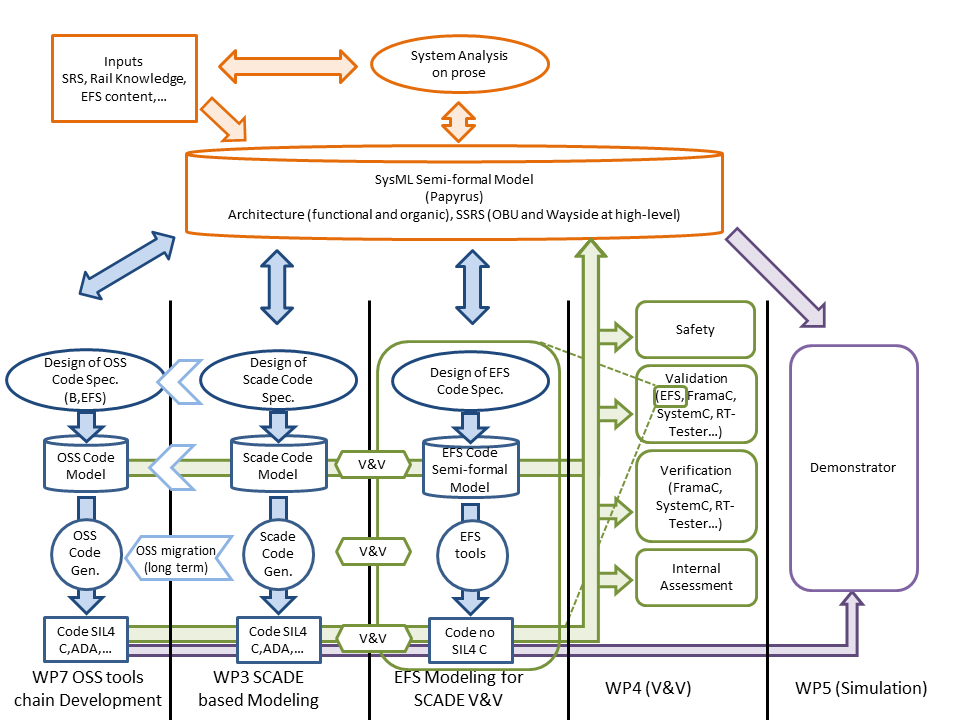
\includegraphics[width=\linewidth]{images/2013_08_28_Toolchain_proposal.png}
  \caption{Proposal for putting the various tools to use.}
  \label{fig:proposal}
\end{figure}

A toolchain proposal had been made by Matthieu Perin, shown in Figure \ref{fig:proposal}.  This proposal was generally met with agreement (discussed in issue \#144, see core idea E-3).

In particular, this approach is interesting with the respect to EFS, as its main objective would become supporting V\&V activities.  However, should there be a problem with the primary toolchain, this would still allow EFS to be used as the main model.  This approach makes EFS complementary (rather than competing) to the primary toolchain and allows openETCS to take advantage of the existing modeling that has already been done with EFS.

\decision{EFS activities will be coordinated with WP4, to support V\&V activities (as these are modeling activities, they still belong in WP3).  This issue must be raised and resolved with the PCC.}{d:efs_vv}

Further, Matthieu proposes to use SCADE to be the primary toolchain.  This is based on core idea S-4, that Scade is the only viable option to get started NOW.  Note that this point of view is dominating, but by no means universal.  There are proponents for B and EFS, who will still be able to influence this decision, as outlined by Decision~\ref{d:deadline}.

This also means that Decision~\ref{d:sysml_validator} must be performed in a way to take the constraints of the  SCADE Papyrus model into account.

\decision{Unless new evidence is provided in agreement with Decision~\ref{d:deadline}, SCADE will be considered the foundation for the primary toolchain.  In that case, a feasible migration from what had been done with SCADE is essential.}{d:scade}

SCADE two major drawbacks: (1) it is not open source, and (2) it is very expensive (core idea S-3).  Figure~\ref{fig:proposal} addresses the first issue, which is also recorded in core idea S-1, by proposing an OSS migration to a B or EFS-based toolchain.  In fact, as outlined in Decision~\ref{d:scade}, this migration may happen much sooner, if evidence is presented. 

\decision{Work on the toolchain must always take the objective of an OSS migration into account, e.g. by standardizing interfaces between tools.  It is acknowledged that such a migration may not be feasible within the timeframe of the openETCS project.  However, by the end of the project, feasibility of a migration must be demonstrated (e.g. with a prototype or case study).}{d:oss}

The second issue can only be resolved in collaboration with Esterel, the manufacturer of SCADE.  Klaus-Rüdiger Hase expressed confidence in finding a solution for all parties, after the initial negotiations with Esterel.  To make sure that we won't have a problem in this regard, we formulate the following ``nuclear option'' and will make Esterel aware of it:

\decision{All openETCS project partners must be made aware of the need for acquiring a SCADE license (depending on their activities).  If a partner feels that this is not achievable, this must be escalated to the project office by \textbf{November 15, 2013}.  The project office will assist in finding a solution.  If no solution has been found by January 31, 2014 for all partners who escalated, then SCADE will be abandoned for anything on the critical path of the toolchain.}{d:price}

Last, there are proponents for EFS and B.  While work on EFS will continue, as described in Decision~\ref{d:efs_vv}, we will state explicitly that the B team may continue to investigate the possibilities of its use, in the spirit of a meritocracy.

Outside help for this task may be available, as Polarsys (an Eclipse Industry Working Group) has similar objectives.  The team is strongly advised to coordinate with them. This is reflected in core idea O-5.

\decision{According to the spirit of an open proofs project, team members are permitted to continue evaluating B, even with the objective of contradicting Decision~\ref{d:scade}.  However, if unsuccessful by the deadline set by Decision~\ref{d:deadline}, they must refocus either by contributing elsewhere, or by focusing on the transition to OSS, as outlined in Figure~\ref{fig:proposal}\footnotemark.  The team is strongly encouraged to coordinate with Polarsys.}{d:b}

\footnotetext{This decision assumes that the WP leader has managerial authority over the work package's resources (and consequently, that these activities are coordinated with WP leadership).  If it turns out that this is not the case, then this aspect of the decision will be void.  This is currently investigated and documented in \url{https://github.com/openETCS/governance/issues/60}.}
\section{Recommendations for WP3 Modeling}

We can make decisions for WP7, but can only articulate recommendations for WP3.  Making these will hopefully clarify the intentions behind our decisions even more.

While the decisions document that for now, SCADE and Papyurus will be the foundation for the primary tool chain, we strongly recommend to focus on Papyrus and to do as little work with the SCADE tools.  There are still many discussions ahead, also with respect to the secondary tooling.  Thus, the longer the decision can be delayed, the better.  It will also allow the D2.4 team to provide a development method.

\section{Conclusion}

Reaching the decisions documented here was the result of the constructive collaboration of a large number of partners.  We believe that we decided on an approach that will allow WP3 and WP4 to confidently pursue their activities (modeling and V\&V, respectively), while still leaving room to adjust course within the next six months.  The decisions lay the groundwork for building an open proofs toolchain.  However, should we not manage to achieve this ambitious goal, this will not jeopardize the project.

The previous section \ref{sec:dec} gives the actual decisions taken by WP7 and project partners.
However, decisions or points of view have been given by the leaders of other workpackages and are summed up in the sequel.

\subsection{WP3 point of view}

Point of view of WP3 leader, taken from issue \#109):

\begin{quote}
Indeed, ALSTOM, as modeling WP leader, needs now to organize WP3 kick-off meeting and ressources working within a clear framework and objective. With D7.1 conclusion as it is now, WP3 ressources are working now in the tools they want to work on without clear strategy nore objective.
Therefore, ALSTOM proposed following D7.1 conclusions to be:

\begin{enumerate}
\item Despite the fact it is not fully open tools, ``SYSML / SCADE'' is the baseline primary tools chain to be used for any modeling activity within the frame of the OpenETCS project unless other agreement and.or decision not late than January 2014.

\item In order to allow availability of another complete full OpenETCS Tools chain, complementary analysis and work will be carried out on the 2 other options ``SYSML/EFS/Eclipse Polarys'' and ``SYSML / Classical B'' for final decision on "OpenETCS" Tools chain not late than January 2014
\end{enumerate}

Such conclusion is likely to avoid dispersion of WP3 ressources that lead to impossibility to manage modeling WP while keeping intact the possibility for the other candidate tools chain to be adopted if confirmed as complete and usable as the only today's available fitted for purpose ``SYSML / SCADE'' solution.
\end{quote}

\subsection{WP4 point of view}

Some decisions have been made by the WP4 partners regarding VnV and safety activities. these decision have been announced during the decision in Paris on July 4th, 2013:

\decision{WP4 is going to consider the artifacts of "SysML+ Scade" toolchain for the first round of verification and validation launched in July 2013.}{d:wp4_scade}

\decision{For the following rounds, starting in February 2014, WP4 will adapt the verification and validation activities to the models and code provides by WP3.}{d:wp4_future}


